%% ΕΛΕΓΧΟΣ ΣΥΣΤΗΜΑΤΟΣ
%% Το μέρος του εγγράφου αυτού περιέχει την περιγραφή της διαδικασίας
%% ελέγχου που χρησιμοποιείθηκε για την διασφάλιση της σωστής λειτουργίας
%% της εφαρμογής.

\chapter{Έλεγχος Συστήματος}
Σε κάθε τομέα παραγωγής προϊόντων είναι πολύ σημαντικό να παράγονται προϊόντα τα οποία να τηρούν πάντα τις προδιαγραφές τους και να μπορούν να αντεπεξέλθουν στις απαιτήσεις του καταναλωτικού κοινού. Η φήμη και η εμπιστοσύνη που προσδίδει μια εταιρεία είναι κομβικά χαρακτηριστικά για την βιωσιμότητας της. Κάθε επαγγελματίας είναι απαραίτητο να είναι σε θέση να εγγυηθεί για την ποιότητα του προϊόντος ή της υπηρεσίας που παρέχει ως αντάλλαγμα της αμοιβής του.

Ο τρόπος διασφάλισης της ποιότητας διαφέρει ανάλογα με την φύση του προϊόντος ή της υπηρεσίας και μπορεί να εκτελεστεί με διάφορους μεθόδους. Για παράδειγμα αν το προϊόν ήταν κάποιο τρόφιμο η εταιρία θα έπρεπε να είναι σίγουρη ότι είναι σε άριστη κατάσταση πριν φτάσει στο τραπέζι του καταναλωτή, διότι αν δεν το έκανε αυτό θα υπήρχαν επιπλοκές στην υγεία των καταναλωτών. Αντίστοιχα μια εταιρία που παρέχει μια υπηρεσία πρέπει να διασφαλίσει και να ελέγξει την ποιότητα παροχής της υπηρεσίας με διάφορους τρόπους. Ένας από αυτούς θα ήταν να λαμβάνει τις παρατηρήσεις των καταναλωτών αφότου λάβουν την υπηρεσία ή να περνάει από εσωτερικές εξετάσεις και εκπαίδευση τους υπαλλήλους της έτσι ώστε να είναι σίγουρη ότι αυτοί θα μπορούν να παρέχουν σωστά και αξιόπιστα την υπηρεσία στους πελάτες.

Στην διαδικασία ανάπτυξης λογισμικού υπάρχουν αντίστοιχα διάφοροι τρόποι ελέγχου ότι το λογισμικό που αναπτύσσεται τηρεί τις προδιαγραφές του. Κάποιοι από αυτούς τους τρόπους είναι τα unit testing, fuzz testing, δημοσίευση δοκιμαστική έκδοσης (beta version) κ.α. Το πιο κοντινό εργαλείο ελέγχου στον προγραμματιστή είναι η διαδικασία unit testing η οποία εφαρμόζεται αποκλειστικά σε αντικειμενοστραφή κώδικα. Παρακάτω θα γίνει μια ανάλυση αυτής της τεχνικής ελέγχου και θα αναφερθούν οι μέθοδοι και η διαδικασία ελέγχου πάνω στο Easy!Appointments.

\section {Unit testing}
Για την υλοποίηση unit tests πάνω στον κώδικα είναι απαραίτητο να τηρούνται δύο πράγματα: (1) η αντικειμενοστραφείς δομή και (2) η χρήση κάποιας βιβλιοθήκης ή εργαλείου το οποίο μπορεί να βοηθήσει στην οργάνωση και καλύτερη υλοποίηση των tests.

Με τον όρο unit testing εννοείται η δοκιμή μίας “λειτουργικής μονάδας” του λογισμικού που αναπτύσσεται. Η κάθε λειτουργική μονάδα απομονώνεται από τις υπόλοιπες και δοκιμάζεται ξεχωριστά σε διάφορες καταστάσεις. Για αυτόν τον λόγο είναι απαραίτητο ο κώδικας να έχει αντικειμενοστραφής δομή. Η διαδικασία χωρίζεται στην συγγραφή πολλαπλών unit test, συναρτήσεων δηλαδή που δοκιμάζουν μια διαδικασία για συγκεκριμένες τιμές εισόδου. Σε κάθε περίπτωση στόχος είναι να υπάρχει ελεγχόμενη έξοδος έτσι ώστε να μπορέσει ο προγραμματιστής να είναι σίγουρος ότι το σύστημα θα λειτουργήσει σωστά σε οποιαδήποτε κατάσταση και αν βρίσκεται. Κατά την διαδικασία αυτήν μπορούν να βρεθούν πολύ εύκολα πολλά προβλήματα και ασυνέπειες στον κώδικα ενός συστήματος, τα οποία χρειάζεται να αντιμετωπιστούν. 

Για να μπορέσουν να υλοποιηθούν αυτά τα test είναι απαραίτητο να χρησιμοποιηθεί κάποια βιβλιοθήκη ή εργαλείο το οποίο θα κατέχει τις βασικές συναρτήσεις ελέγχου αποτελεσμάτων και επιπρόσθετα λειτουργίες για την παραγωγή αναφορών, οι οποίες περιέχουν τα αποτελέσματα των δοκιμών. Υπάρχουν πάρα πολλά εργαλεία που κάνουν αυτήν την δουλειά, το καθένα για μια συγκεκριμένη γλώσσα προγραμματισμού. Τα πιο διαδεδομένα εργαλεία είναι αυτά που ανήκουν στην οικογένεια xUnit (JUnit, CppUnit, NUnit κ.α).

Τα εργαλεία αυτά μπορούν συνήθως κάλλιστα να συνεργαστούν μαζί με άλλα εργαλεία ανάπτυξης έτσι ώστε να είναι πολύ εύκολο για τον προγραμματιστή να συμπεριλάβει την διαδικασία unit testing στην υλοποίηση του κάθε συστήματος.

\section {Easy!Appointments testing}
Η συγγραφή των unit tests για το Easy!Appointments έγινε με την χρήση της ενσωματωμένης βιβλιοθήκης που παρέχει το CodeIgniter. Η βιβλιοθήκη παρέχει τις βασικές λειτουργίες ελέγχου και παραγωγής αναφορών για τα tests του κώδικα. Προτιμήθηκε έναντι του phpunit λόγω της καλύτερης απόδοσης σε σχέση με το CodeIgniter Framework. 

Η διαδικασία της δοκιμής του συστήματος ξεκίνησε από τα models, τις λειτουργικές μονάδες που διαχειρίζονται την κίνηση των δεδομένων προς και από την βάση δεδομένων. Είναι απαραίτητο για το σύστημα να κατέχει ακέραια δεδομένα μιας και όλη η εφαρμογή βασίζεται σε αυτά. Η κάθε μέθοδος του κάθε model δοκιμάστηκε ξεχωριστά από τις υπόλοιπες για 3-5 διαφορετικές περιπτώσεις. Όσο αναπτύσσεται το σύστημα τόσο αυξάνονται και unit tests.

\begin{figure}[h]
\centering
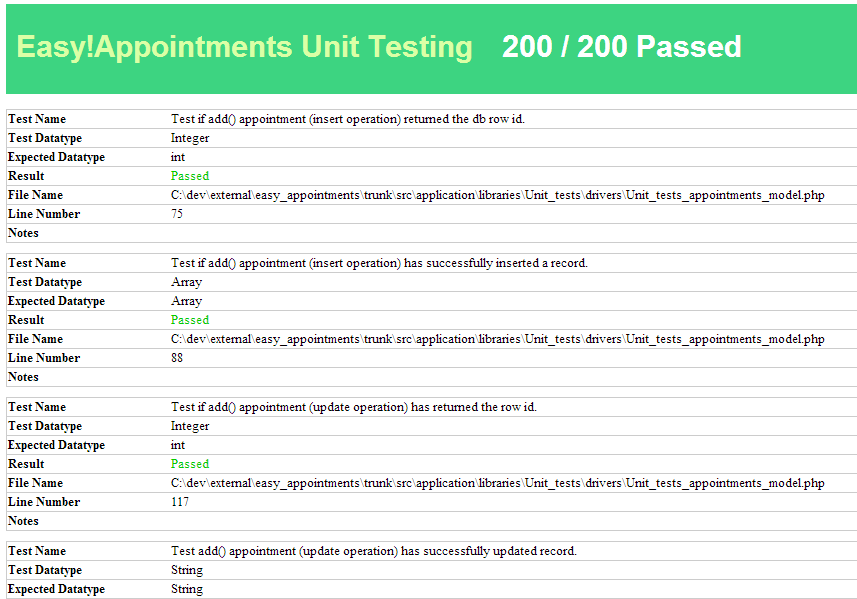
\includegraphics[width=150mm]{images/ea-unit-testing.png}
\caption{Στιγμιότυπο της σελίδας εμφάνισης αποτελεσμάτων των unit tests.}
\label{ea-unit-testing}
\end{figure}

Για να γίνει αυτόματη εκτέλεση όλων των unit test που αντιστοιχούν σε ένα συγκεκριμένο model γράφτηκε η παρακάτω μέθοδος η οποία αφού ελέγξει τα ονόματα των test μεθόδων, εκτελεί μόνο εκείνα τα οποία ξεκινούν από την λέξη "test". Έτσι αν κάποια μέθοδος δεν είναι έτοιμη ή δεν πρέπει να συμπεριληφθεί στην εκτέλεση των unit test αρκεί να αλλάξει την αρχή του ονόματος της και η μέθοδος δεν θα την λάβει υπόψιν.

\lstinputlisting{snippets/unit_test_automation.php} 

\section {Παραδείγματα} 
Στον παρακάτω κώδικα δοκιμάζεται η βασική ροή της περίπτωσης χρήσης “προσθήκη ραντεβού”. Σε αυτό το test case η είσοδος της μεθόδου add() είναι σωστή και αναμένεται ότι και το αποτέλεσμα της διαδικασίας θα είναι επιτυχές. Στο τέλος αφαιρείται η εγγραφή που προστέθηκε για να μην μείνουν κατάλοιπα στην βάση. Σε κάθε unit test χρησιμοποιείται μόνο μια μέθοδος του model. Έτσι το κάθε test δεν επηρεάζεται από τυχόν προβλήματα σε άλλες μεθόδους του model.

\lstinputlisting{snippets/unit_test_insert_example.php}

Στο παρακάτω unit test δοκιμάζεται η μέθοδος get\_value() η οποία επιστρέφει την τιμή ενός πεδίου από την βάση. Στο συγκεκριμένο test case δίνεται ως παράμετρος ένα id εγγραφής το οποίο δεν υπάρχει στην βάση. Η αναμενόμενη συμπεριφορά από το model είναι να εμφανιστεί ένα exception το οποίο να ειδοποιεί ότι η εγγραφή με το συγκεκριμένο id δεν βρέθηκε στην βάση.

\lstinputlisting{snippets/unit_test_get_value_example.php}

Κάποια unit test δοκιμάζουν τις μεθόδους για σωστές τιμές και αναμένουν την επιτυχή ολοκλήρωση των διαδικασιών τους. Τα περισσότερα όμως tests σκοπό έχουν να δουν την συμπεριφορά του συστήματος για τιμές οι οποίες δεν είναι φυσιολογικές. Με αυτόν τον τρόπο μπορούν να προβλεφθούν πολλά bug και άλλα προβλήματα στον κώδικα και η εφαρμογή να είναι περισσότερο αξιόπιστη και δυνατή απέναντι σε σφάλματα.